\section{Analysis and Design}

\subsection{Requirements}
The requirements below describe the visible behaviour and architectural constraints verified in the
Rùa Toán Basic application.

\subsubsection{Functional requirements}
\begin{enumerate}[label=FR\arabic*.]
  \item \textbf{Curated exam collections:} Browse 3,381 collections with pagination (20 per page) and open
        a collection to inspect nested problems in original chronological order with source attribution and external links.
  \item \textbf{Practice problem discovery:} Search and filter 33,929 individual problems by grade (6--10),
        mathematical topic, and text keyword using Vietnamese diacritic-insensitive matching.
  \item \textbf{Mathematical notation typesetting:} Dynamically render inline (\texttt{\$...\$}) and display
        (\texttt{\$\$...\$\$}) LaTeX notation in problem statements, hints, and lesson bodies using MathJax 3.
  \item \textbf{Theory and library catalogue:} Browse 90 structured lessons across five mathematical domains with
        client-side search and accordion expansion; access 216 books and 89 documents with source links.
  \item \textbf{User authentication:} Register, authenticate, change password, and safely log out with email
        and password, holding authenticated state in an HMAC-signed \texttt{HttpOnly} cookie.
  \item \textbf{Single-use password recovery:} Request a time-bounded (30-minute) cryptographically secure password
        reset token persisted in PostgreSQL, enabling account recovery without third-party email dependencies.
  \item \textbf{Homework photo submissions:} Upload up to six written work photos (1.5 MB each) per submission,
        preview existing submissions in a thumbnail gallery, and securely delete owned submissions.
  \item \textbf{Local problem bookmarking:} Save and remove marked problems locally via
        browser \texttt{localStorage}, persisting selections without an account.
  \item \textbf{Catalogue metrics:} Present live content totals (problems, collections, lessons, books, documents)
        on the home page fetched dynamically from the backend.
\end{enumerate}

\subsubsection{Non-functional requirements and constraints}
\begin{itemize}
  \item \textbf{Responsive multi-device layout:} Pages must render cleanly across mobile viewports (down to 390~px)
        and desktop displays (up to 1440~px) using responsive CSS Grid and Flexbox without framework overhead.
  \item \textbf{First-principles inspectability:} The client bundle must contain zero compiled/minified artifacts
        or node module dependencies; every HTML, CSS, and JS file must be directly inspectable in browser DevTools.
  \item \textbf{Serverless performance and connection efficiency:} The FastAPI backend running on Vercel
        must enforce connection pooling to avoid PostgreSQL connection starvation under concurrent edge requests.
  \item \textbf{Bounded file upload security:} The backend must enforce file size limits (1.5 MB/file, max 6 files)
        and inspect binary magic bytes (PNG, JPEG, WebP) to prevent arbitrary file upload vulnerabilities.
  \item \textbf{Password security:} Passwords must be hashed using PBKDF2-HMAC-SHA256 with 200,000 iterations
        and a 16-byte random cryptographic salt; password inputs are bounded to 128 characters to prevent CPU exhaustion.
  \item \textbf{Web accessibility (a11y):} Form controls must have high-contrast borders and backgrounds in both
        light and dark modes; interactive elements must present prominent keyboard focus rings (\texttt{:focus-visible}).
  \item \textbf{Stateless session confidentiality:} Session cookies must use \texttt{HttpOnly}, \texttt{SameSite=Lax},
        and \texttt{Secure} flags, with cryptographic HMAC-SHA256 signatures to prevent client-side tampering.
\end{itemize}

\subsection{Interface design (UI/UX)}
The visual identity of Rùa Toán Basic embodies an authentic, tactile mathematics workshop theme designed
for readability and low visual fatigue during extended problem solving:
\begin{itemize}
  \item \textbf{Color palette tokens:} Grounded in a deep forest green primary background (\texttt{\#0F3D2E}, \texttt{--bg}),
        dark pine operational panels (\texttt{\#163523}, \texttt{--card}), and high-contrast parchment paper cards
        (\texttt{\#FFF8E7}, \texttt{--surface}) optimized for rendering crisp mathematical symbols and text.
  \item \textbf{Turtle-themed playful accents:} Vibrant slime lime (\texttt{\#B6FF3B}, \texttt{--ooze}) for active
        states and call-to-action buttons; warm amber (\texttt{\#FBB03B}) for badges and metrics; and terracotta coral
        (\texttt{\#FF6F59}) for warnings and remove actions.
  \item \textbf{Typography hierarchy:} Google Font \textbf{Bungee} is employed for retro, playful headings, collection
        badges, and numeric counters, evoking a gamified learning atmosphere; \textbf{Be Vietnam Pro} serves as the
        primary body typeface for highly legible Vietnamese typography and mathematical explanations.
  \item \textbf{Tactile 3D components:} Collection and problem cards feature distinct 3D neomorphic drop-shadow
        borders (\texttt{3px solid var(--ink)} with offset \texttt{4px 4px 0 var(--ink)}), delivering satisfying
        tactile feedback upon click and focus.
  \item \textbf{Uniform modular page structure:} Every page shares a consistent, recognizable skeleton:
        \texttt{top/header} (brand logo, navigation links, session badge), \texttt{phead} (hero title and subheadings),
        \texttt{topics} (filter pills for grades 6--9 and math branches), \texttt{grid/ccard} (cards feed),
        \texttt{pager} (pagination bar), and \texttt{foot} (credits, GitHub repository link, license).
\end{itemize}
The complete suite of production interface screenshots is presented and discussed in Section~\ref{sec:ui-implementation}.

\subsection{System architecture}
Figure~\ref{fig:architecture} illustrates the system architecture of Rùa Toán Basic. The architecture
separates static delivery from dynamic computation and durable database storage:
\begin{itemize}
  \item \textbf{Client browser:} Executes plain JavaScript (ES2020) to handle user events, manages client-side
        bookmarking in \texttt{localStorage}, renders mathematical expressions via MathJax, and dispatches
        asynchronous JSON requests to RESTful endpoints.
  \item \textbf{Vercel Edge CDN:} Distributes static assets (\texttt{public/index.html}, \texttt{public/pages/*},
        CSS stylesheets, JS modules, images) directly from global edge caches with zero serverless cold-start latency.
  \item \textbf{FastAPI Serverless Function:} The Python ASGI entry point (\texttt{main.py}) handles API routes
        under \texttt{/api/*}. It maintains an in-memory cached view of the JSON catalogue and manages session cookies.
  \item \textbf{PostgreSQL Database:} Hosted durably in cloud infrastructure, storing user accounts, password
        reset tokens, and binary photo data in dedicated schema \texttt{ruatoan\_basic}.
\end{itemize}

\begin{figure}[ht]
\centering
\begin{tikzpicture}[
  box/.style={draw=PrussianBlue,fill=PaleBlue,rounded corners=2pt,align=center,text width=3.2cm,minimum height=1.15cm},
  data/.style={draw=FDABlue,fill=Solitude,rounded corners=2pt,align=center,text width=3.6cm,minimum height=1.1cm},
  arrow/.style={->,thick,color=PrussianBlue}
]
\node[box] (browser) at (0,0) {\textbf{Student Browser}\\Plain HTML5 / CSS3 / JS\\MathJax 3; localStorage};
\node[box] (vercel) at (5.2,0) {\textbf{Vercel Serverless}\\Static files from \texttt{public/}\\FastAPI ASGI for \texttt{/api/*}};
\node[data] (json) at (10.6,1.6) {\textbf{Catalogue JSON}\\3,381 collections\\33,929 problems, 90 lessons};
\node[data] (pg) at (10.6,-1.6) {\textbf{PostgreSQL Database}\\\small\texttt{ruatoan\_basic.users}\\\footnotesize\texttt{ruatoan\_basic.photos}};
\draw[arrow,<->] (browser) -- (vercel);
\draw[arrow] (vercel) -- (json);
\draw[arrow,<->] (vercel) -- (pg);
\end{tikzpicture}
\caption{System architecture of Rùa Toán Basic showing separation between static CDN assets, serverless API execution, in-memory JSON catalogue, and durable PostgreSQL storage.}
\label{fig:architecture}
\end{figure}

\subsection{Database design}
PostgreSQL is utilized specifically for mutable application state: registered user accounts,
cryptographic password reset tokens, and homework photographs. The application isolates its tables
within the \texttt{ruatoan\_basic} schema to avoid namespace collisions with any existing databases.
The entity relationships and schema specifications are illustrated in Figure~\ref{fig:er-diagram}.

\begin{figure}[ht]
\centering
\begin{tikzpicture}[
  entity/.style={draw=PrussianBlue,fill=Solitude,rounded corners=3pt,align=left,font=\small,inner sep=7pt},
  arrow/.style={->,thick,color=PrussianBlue}
]
\node[entity] (users) at (0,0) {
  \textbf{users}\\
  \rule{4.2cm}{0.4pt}\\
  \textbf{\underline{id}} : VARCHAR(36) [PK]\\
  name : VARCHAR(80)\\
  email : VARCHAR(255) [UNIQUE]\\
  password\_hash : VARCHAR(255)\\
  created\_at : TIMESTAMPTZ
};

\node[entity] (photos) at (6.8,1.6) {
  \textbf{photos}\\
  \rule{4.6cm}{0.4pt}\\
  \textbf{\underline{id}} : VARCHAR(36) [PK]\\
  \textit{user\_id} : VARCHAR(36) [FK $\to$ users.id]\\
  file\_name : VARCHAR(255)\\
  content\_type : VARCHAR(50)\\
  byte\_size : INTEGER\\
  data : BYTEA\\
  created\_at : TIMESTAMPTZ
};

\node[entity] (resets) at (6.8,-1.8) {
  \textbf{password\_resets}\\
  \rule{4.6cm}{0.4pt}\\
  \textbf{\underline{id}} : VARCHAR(36) [PK]\\
  \textit{user\_id} : VARCHAR(36) [FK $\to$ users.id]\\
  token\_hash : VARCHAR(64) [UNIQUE]\\
  expires\_at : TIMESTAMPTZ\\
  created\_at : TIMESTAMPTZ
};

\draw[arrow] (users.east) -- node[above,font=\footnotesize] {1 : N (CASCADE)} (photos.west);
\draw[arrow] (users.east) -- node[below,font=\footnotesize] {1 : N (CASCADE)} (resets.west);
\end{tikzpicture}
\caption{Entity-Relationship (ER) diagram for PostgreSQL schema \texttt{ruatoan\_basic}. Cascading foreign keys preserve database integrity upon account deletion.}
\label{fig:er-diagram}
\end{figure}

\textbf{Durable binary storage vs. ephemeral filesystems.}
Serverless execution environments on platforms like Vercel provide only a short-lived, read-only
or temporary container filesystem (\texttt{/tmp}) that is destroyed when the function container spins down.
Consequently, homework photographs cannot be stored on the local filesystem. Rùa Toán Basic stores
validated image data directly in the \texttt{photos.data} column as PostgreSQL \texttt{BYTEA} binary data.
This architecture guarantees data durability without requiring expensive external cloud object storage (such as AWS S3)
for the scope of this project.

\subsection{Data design}
The curriculum content is organized into versioned JSON files directly within the repository.
The groups and record distributions are summarized in Table~\ref{tab:data-groups}.
The static corpus comprises 11 exam collection files (\texttt{data/sources/}), 7 theory files
(\texttt{data/theory/}), and reference files \texttt{books.json} and \texttt{docs.json}, totaling ~16 MB on disk.

\begin{table}[ht]
\centering\small
\begin{tabularx}{\textwidth}{@{}l r >{\raggedright\arraybackslash}X@{}}
\toprule
\textbf{Record group} & \textbf{Count} & \textbf{Primary fields and purpose}\\
\midrule
Collections & 3,381 & ID, kind, title, grade, year, province, source name/URL, ordered problems\\
Problems & 33,929 & ID, label, statement text, topic tags; nested inside collections\\
Lessons & 90 & ID, topic area, title, summary, LaTeX body, examples\\
Books and resources & 216 & ID, title, author/publisher, target grades, description, URL\\
Documents & 89 & ID, topic, title, author, grade metadata, description, PDF links\\
\bottomrule
\end{tabularx}
\caption{Catalogue groups and record counts verified from the JSON corpus.}
\label{tab:data-groups}
\end{table}

\begin{figure}[ht]
\centering
\begin{tikzpicture}[
  entity/.style={draw=PrussianBlue,fill=Solitude,rounded corners=2pt,align=left,text width=3.3cm,inner sep=6pt},
  arrow/.style={->,thick,color=PrussianBlue}
]
\node[entity] (collection) at (0,0) {\textbf{Collection JSON}\\ID, kind, title, grade\\year, province\\source name and URL};
\node[entity] (problem) at (4.8,0) {\textbf{Nested Problem JSON}\\ID, label, statement\\topic tags\\array order preserved};
\node[entity] (photo) at (9.6,0) {\textbf{PostgreSQL Photo row}\\UUID, user\_id\\file name, MIME, bytes\\created\_at};
\node[entity] (ref) at (0,-3.1) {\textbf{Reference JSON groups}\\Lessons (90)\\Books/resources (216)\\Documents (89)};
\node[entity] (device) at (4.8,-3.1) {\textbf{Browser local storage}\\Marked-problem list\\Not an account profile};
\node[entity] (user) at (9.6,-3.1) {\textbf{PostgreSQL User row}\\id, name\\email (unique, lower)\\password hash};
\draw[arrow] (collection) -- (problem);
\draw[arrow] (user) -- (photo);
\end{tikzpicture}
\caption{Data model relationships showing storage boundaries: versioned JSON, browser localStorage, and PostgreSQL tables.}
\label{fig:data-model}
\end{figure}

The corpus spans five collection kinds: 1,195 HSG (Gifted Student Olympiad), 501 Grade-10 specialized
entrance, 733 Olympiad competitions, 844 mathematical magazines, and 108 topic-specific collections.
Figures~\ref{fig:collection-kind-chart}, \ref{fig:collection-grade-chart}, and \ref{fig:topic-chart}
illustrate the distribution across kinds, grades, and topic assignments.

\begin{figure}[ht]
\centering
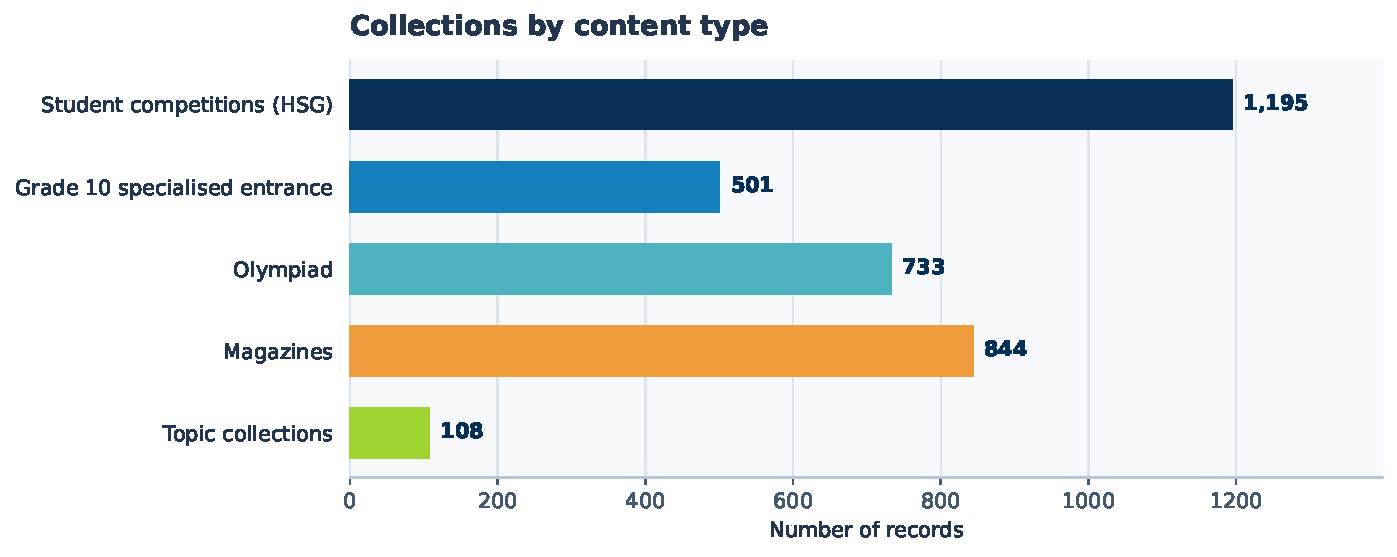
\includegraphics[width=0.88\textwidth]{figures/collection-types.pdf}
\caption{Collection counts by source kind in the curriculum corpus.}
\label{fig:collection-kind-chart}
\end{figure}

\begin{figure}[ht]
\centering
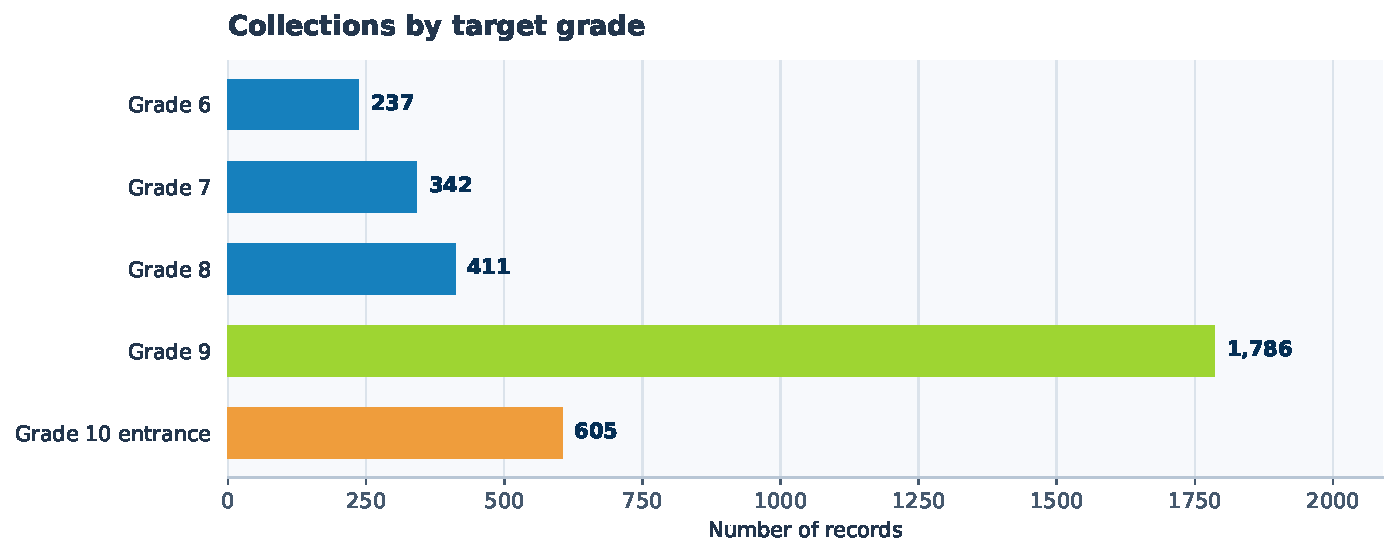
\includegraphics[width=0.88\textwidth]{figures/collection-grades.pdf}
\caption{Collection counts by target grade level (Grade 10 indicates specialized entrance examinations).}
\label{fig:collection-grade-chart}
\end{figure}

\begin{figure}[ht]
\centering
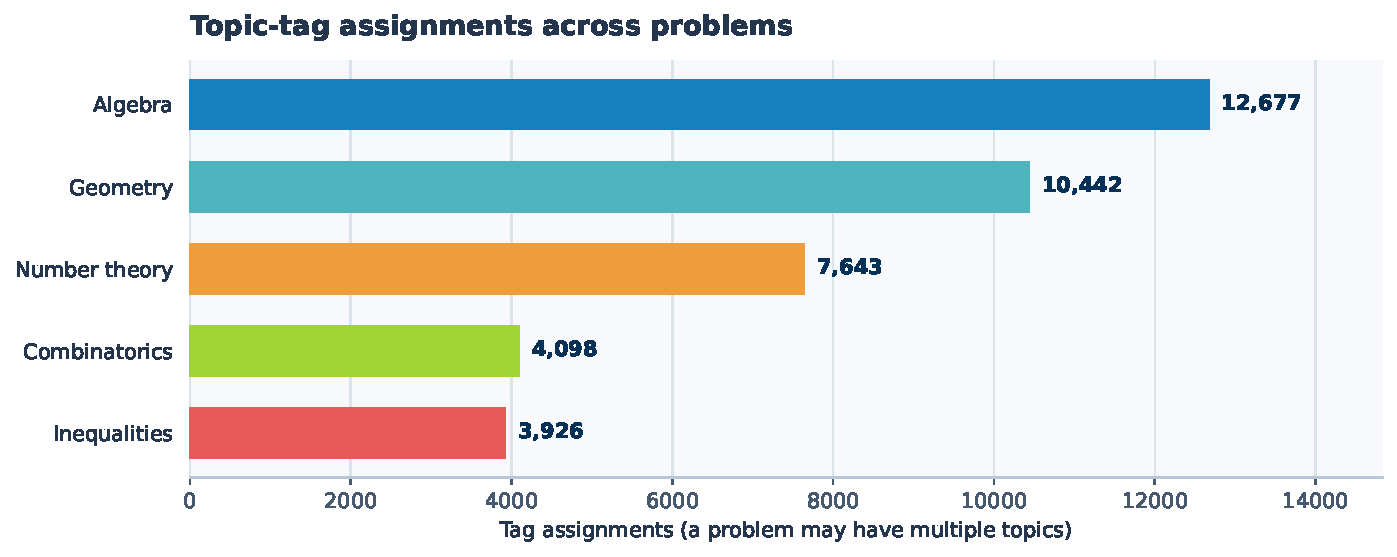
\includegraphics[width=0.88\textwidth]{figures/problem-topic-tags.pdf}
\caption{Topic-tag assignment distribution across problems (multi-tagged problems contribute to multiple bars).}
\label{fig:topic-chart}
\end{figure}

\subsection{API design}
The backend provides a clean RESTful API surface. Table~\ref{tab:api} lists every endpoint, request shape,
and verified HTTP response codes.

\begin{table}[ht]
\centering\footnotesize
\begin{tabularx}{\textwidth}{@{}l l >{\raggedright\arraybackslash}X >{\raggedright\arraybackslash}X@{}}
\toprule
\textbf{Method} & \textbf{Path} & \textbf{Request parameters} & \textbf{Successful result / explicit errors}\\
\midrule
GET & \texttt{/api/stats} & none & \texttt{\{collections, problems, lessons, books, docs, topics\}}\\
GET & \texttt{/api/daily} & none & \texttt{\{problem, collection\}} for today's daily exercise\\
GET & \texttt{/api/collections} & \texttt{?page,} \texttt{limit,} \texttt{grade,} \texttt{kind,} \texttt{year,} \texttt{search} & \texttt{\{total, page, items\}} (summaries only, fast transfer)\\
GET & \texttt{/api/collections/\{id\}} & \texttt{?page, per} & Full collection metadata + paginated problems; 404 if not found\\
GET & \texttt{/api/problems} & \texttt{?page,} \texttt{limit,} \texttt{search,} \texttt{grade,} \texttt{topic} & \texttt{\{total, page, items\}} using folded diacritic matching\\
GET & \texttt{/api/lessons} & \texttt{?search} & \texttt{\{items\}} theory lesson array\\
GET & \texttt{/api/books} & \texttt{?search} & \texttt{\{items\}} book references array\\
GET & \texttt{/api/docs} & \texttt{?search} & \texttt{\{items\}} document references array\\
POST & \texttt{/api/register} & JSON \texttt{\{name, email, password\}} & \texttt{\{user\}}; 400 validation error, 409 duplicate email\\
POST & \texttt{/api/login} & JSON \texttt{\{email, password\}} & \texttt{\{user\}} + sets HttpOnly cookie; 401 invalid credentials\\
POST & \texttt{/api/logout} & session cookie & Clears session cookie\\
POST & \texttt{/api/change-password} & JSON \texttt{\{old\_password, new\_password\}} & \texttt{\{ok: true\}}; 400 bad length, 401 wrong old password\\
POST & \texttt{/api/request-reset} & JSON \texttt{\{email\}} & \texttt{\{ok: true, token\}}; stores 30-min token hash in DB\\
POST & \texttt{/api/reset-password} & JSON \texttt{\{token, new\_password\}} & \texttt{\{ok: true\}}; 400 expired or invalid token\\
GET & \texttt{/api/me} & session cookie (optional) & \texttt{\{user\}} profile or \texttt{\{user: null\}}\\
GET & \texttt{/api/photos} & session cookie & \texttt{\{items\}} metadata array of owned homework photos\\
POST & \texttt{/api/photos} & multipart \texttt{files} (1--6), session cookie & \texttt{\{items\}}; 400 magic-byte error, 413 file > 1.5MB\\
GET & \texttt{/api/photos/\{id\}} & session cookie & Image binary stream with \texttt{nosniff}; 404 if missing\\
DELETE & \texttt{/api/photos/\{id\}} & session cookie & \texttt{\{ok: true\}}; 404 if unowned\\
\bottomrule
\end{tabularx}
\caption{RESTful API endpoints implemented in Rùa Toán Basic and verified by automated smoke testing.}
\label{tab:api}
\end{table}

\subsection{Security design (added in the improvement pass)}\label{sec:security}
During the collaborative bug-fixing pass, the team identified and fortified several critical security vectors:
\begin{itemize}
  \item \textbf{Strict HTTP response security headers:} Injected via FastAPI middleware:
        \texttt{X-Content-Type-Options: nosniff}, \texttt{X-Frame-Options: DENY},
        \texttt{Referrer-Policy}, and a restrictive Content Security Policy (CSP).
  \item \textbf{Input length constraints:} Enforcing password bounds of 8--128 characters to prevent Denial-of-Service
        (DoS) CPU exhaustion against PBKDF2 hashing functions.
  \item \textbf{Magic-byte MIME verification:} Inspecting binary signatures (PNG, JPEG, WebP) rather than trusting
        client-supplied \texttt{Content-Type} headers.
  \item \textbf{Per-user photo storage quota:} Capping total stored photos at 50 per account to protect database disk capacity.
  \item \textbf{Tamper-proof signed session cookies:} Using HMAC-SHA256 signatures over user IDs with expiration
        timestamps, configured with \texttt{HttpOnly}, \texttt{SameSite=Lax}, and \texttt{Secure} flags on HTTPS.
\end{itemize}
